\clearpage

\section{Data vs. MC Comparison in Preselection Region}
\label{sec:yields}

In this section we compare the data and MC samples passing the selection described in Sec.~\ref{sec:eventSelection}
In the following, the MC is reweighted to match the data distribution of number of reconstructed primary vertices
{\bf FIXME: UPDATE TO 5.1/fb VTX-REWEIGHTING, CURRENTLY USING OUTDATED FUNCTION}. 
The trigger efficiencies of Sec.~\ref{sec:datasets} are applied. In all plots, the last bin contains the overflow.

We begin by counting the inclusive Z yields. Here we require the presence of two selected leptons without
any additional requirements on jets or \MET. In Fig.~\ref{fig:dilmass} the distribution of dilepton invariant
mass in the ee and $\mu\mu$ channels is displayed. In Table~\ref{table:zyields} the yields for selected dilepton
events in the Z mass window are indicated. Good data vs. MC agreement is observed, within the systematic uncertainties
of integrated luminosity (4.5\%), trigger efficiency (3\%), \zjets\ and \ttbar\ cross sections.

\begin{figure}[hbt]
  \begin{center}
	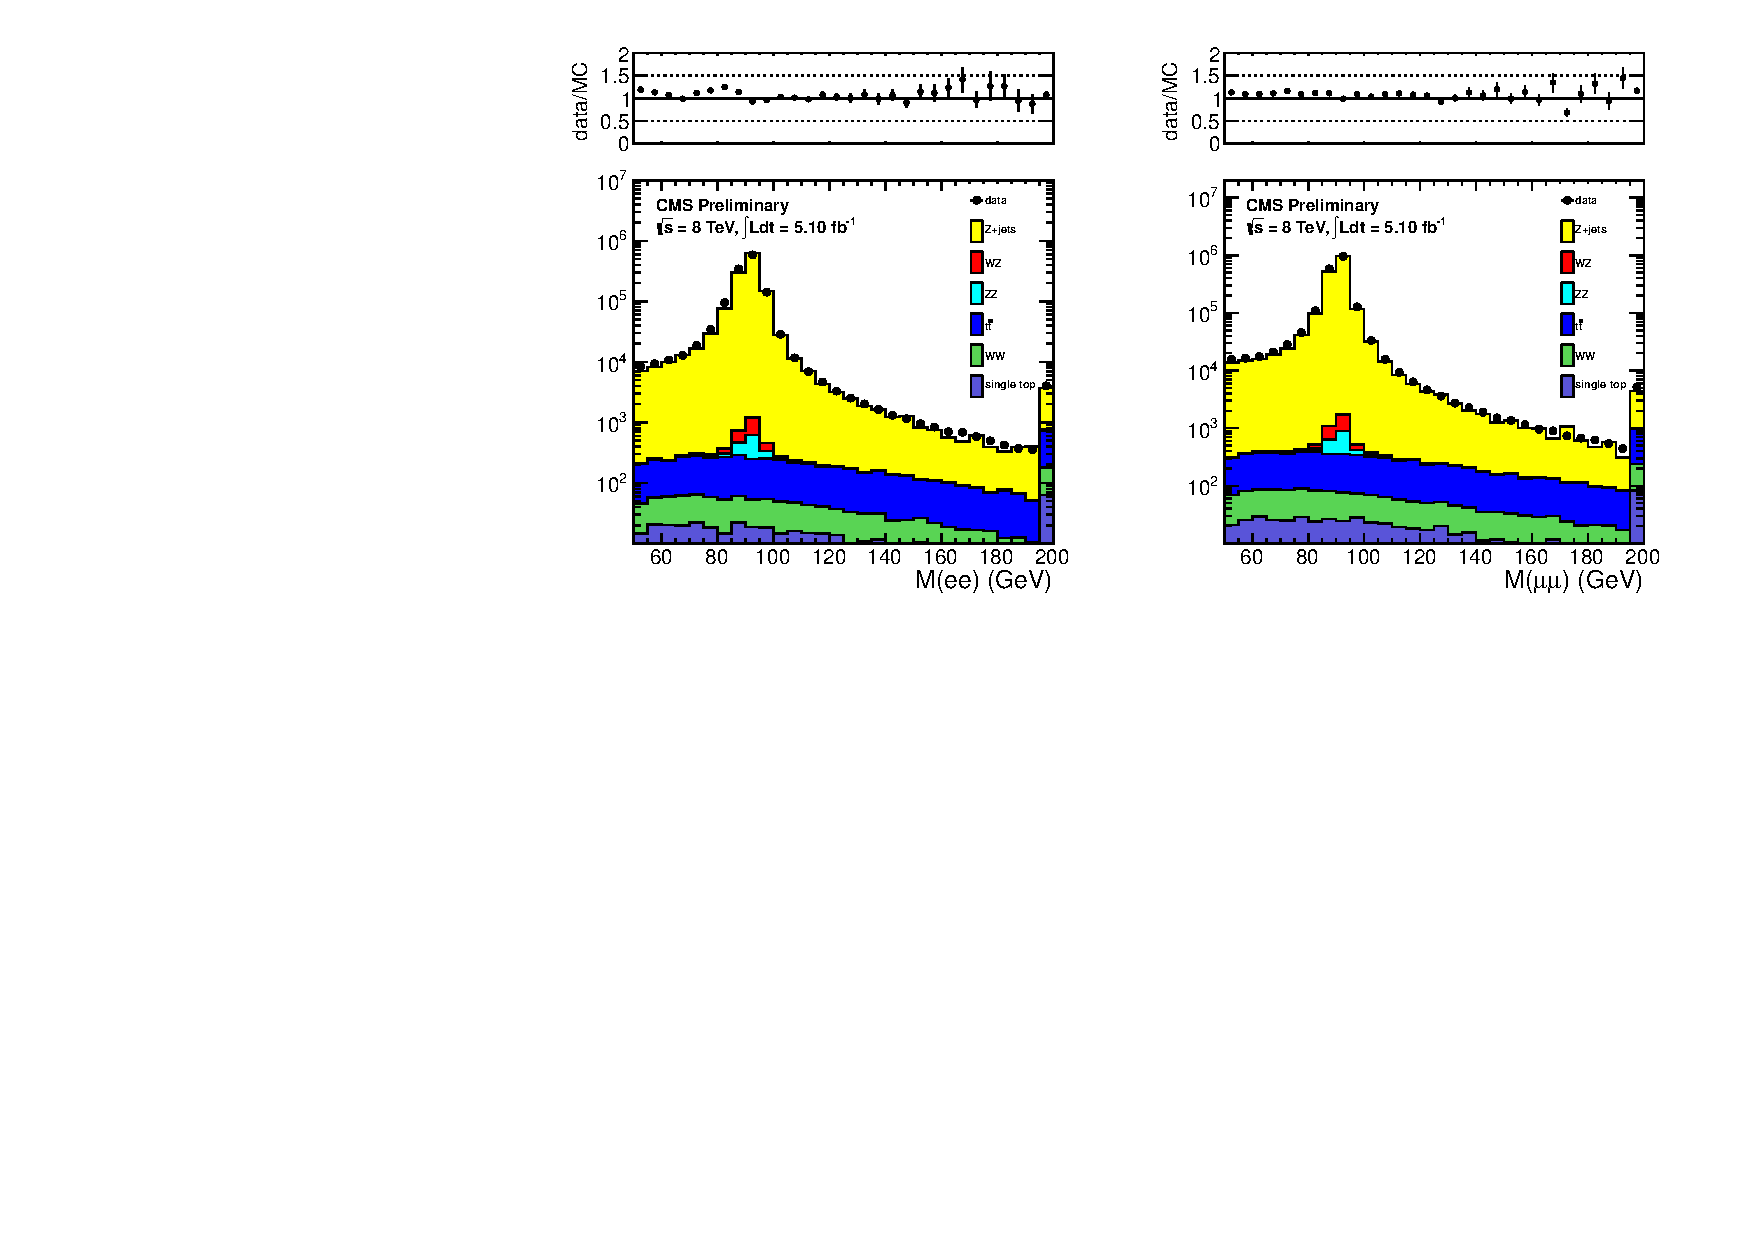
\includegraphics[width=1.0\linewidth]{plots/dilmass_ee_mm.pdf}
	\caption{
	  \label{fig:dilmass}\protect 
	  Dilepton mass distribution for events with two selected leptons
	  in the ee (left) and $\mu\mu$ (right) final states.}
  \end{center}
\end{figure}


\begin{table}[htb]
\begin{center}
\caption{\label{table:zyields} Data and Monte Carlo yields for events with two selected leptons in the Z mass window. 
}
\begin{tabular}{lccccc}
\hline
\hline
              Sample   &                ee   &            $\mu\mu$   &              e$\mu$   &         total         \\
\hline
         \zjets   & 1150211.5 $\pm$ 4886.0   & 1697568.1 $\pm$ 5680.2  &  281.5 $\pm$ 63.7   & 2848061.2 $\pm$ 7492.8  \\
         \ttbar   &     829.1 $\pm$ 20.0     &    1120.7 $\pm$ 22.6    & 1910.9 $\pm$ 29.7   &    3860.7 $\pm$ 42.4    \\
             WZ   &    1038.2 $\pm$ 3.6      &    1465.5 $\pm$ 4.1     &   29.5 $\pm$ 0.5    &    2533.2 $\pm$ 5.5     \\
             ZZ   &     658.0 $\pm$ 2.4      &     933.0 $\pm$ 2.7     &    2.7 $\pm$ 0.1    &    1593.7 $\pm$ 3.6     \\
             WW   &     146.7 $\pm$ 2.6      &     209.0 $\pm$ 2.9     &  358.9 $\pm$ 3.9    &     714.6 $\pm$ 5.5     \\
     single top   &      70.9 $\pm$ 4.9      &     103.3 $\pm$ 5.7     &  172.5 $\pm$ 7.4    &     346.7 $\pm$ 10.5    \\
\hline
    total SM MC   & 1152954.5 $\pm$ 4886.1   & 1701399.6 $\pm$ 5680.3   &2756.1 $\pm$ 70.8   & 2857110.2 $\pm$ 7493.0  \\
           data   &        1162229   &        1774353   &           3077   &        2939659  \\
\hline
\hline
\end{tabular}
\end{center}
\end{table}

\clearpage

We next define the preselection region for the inclusive search using the following requirements:
\begin{itemize}
\item Number of jets $\geq$ 2;
\item Same flavor dileptons (opposite flavor yields will be shown since they are used in data for the FS background estimation);
\item Dilepton invariant mass $81<m_{\ell\ell}<101$ GeV.
\end{itemize}

The dilepton mass distributions in the preselection region of the inclusive search (without the dilepton mass requirement applied) 
for the ee and $\mu\mu$ final states are shown in Figure~\ref{fig:dilmass_2j}. In Table~\ref{table:zyields_2j} the data and MC yields in the preselection
region are indicated. Good data vs. MC agreement is observed.


\begin{figure}[hbt]
  \begin{center}
	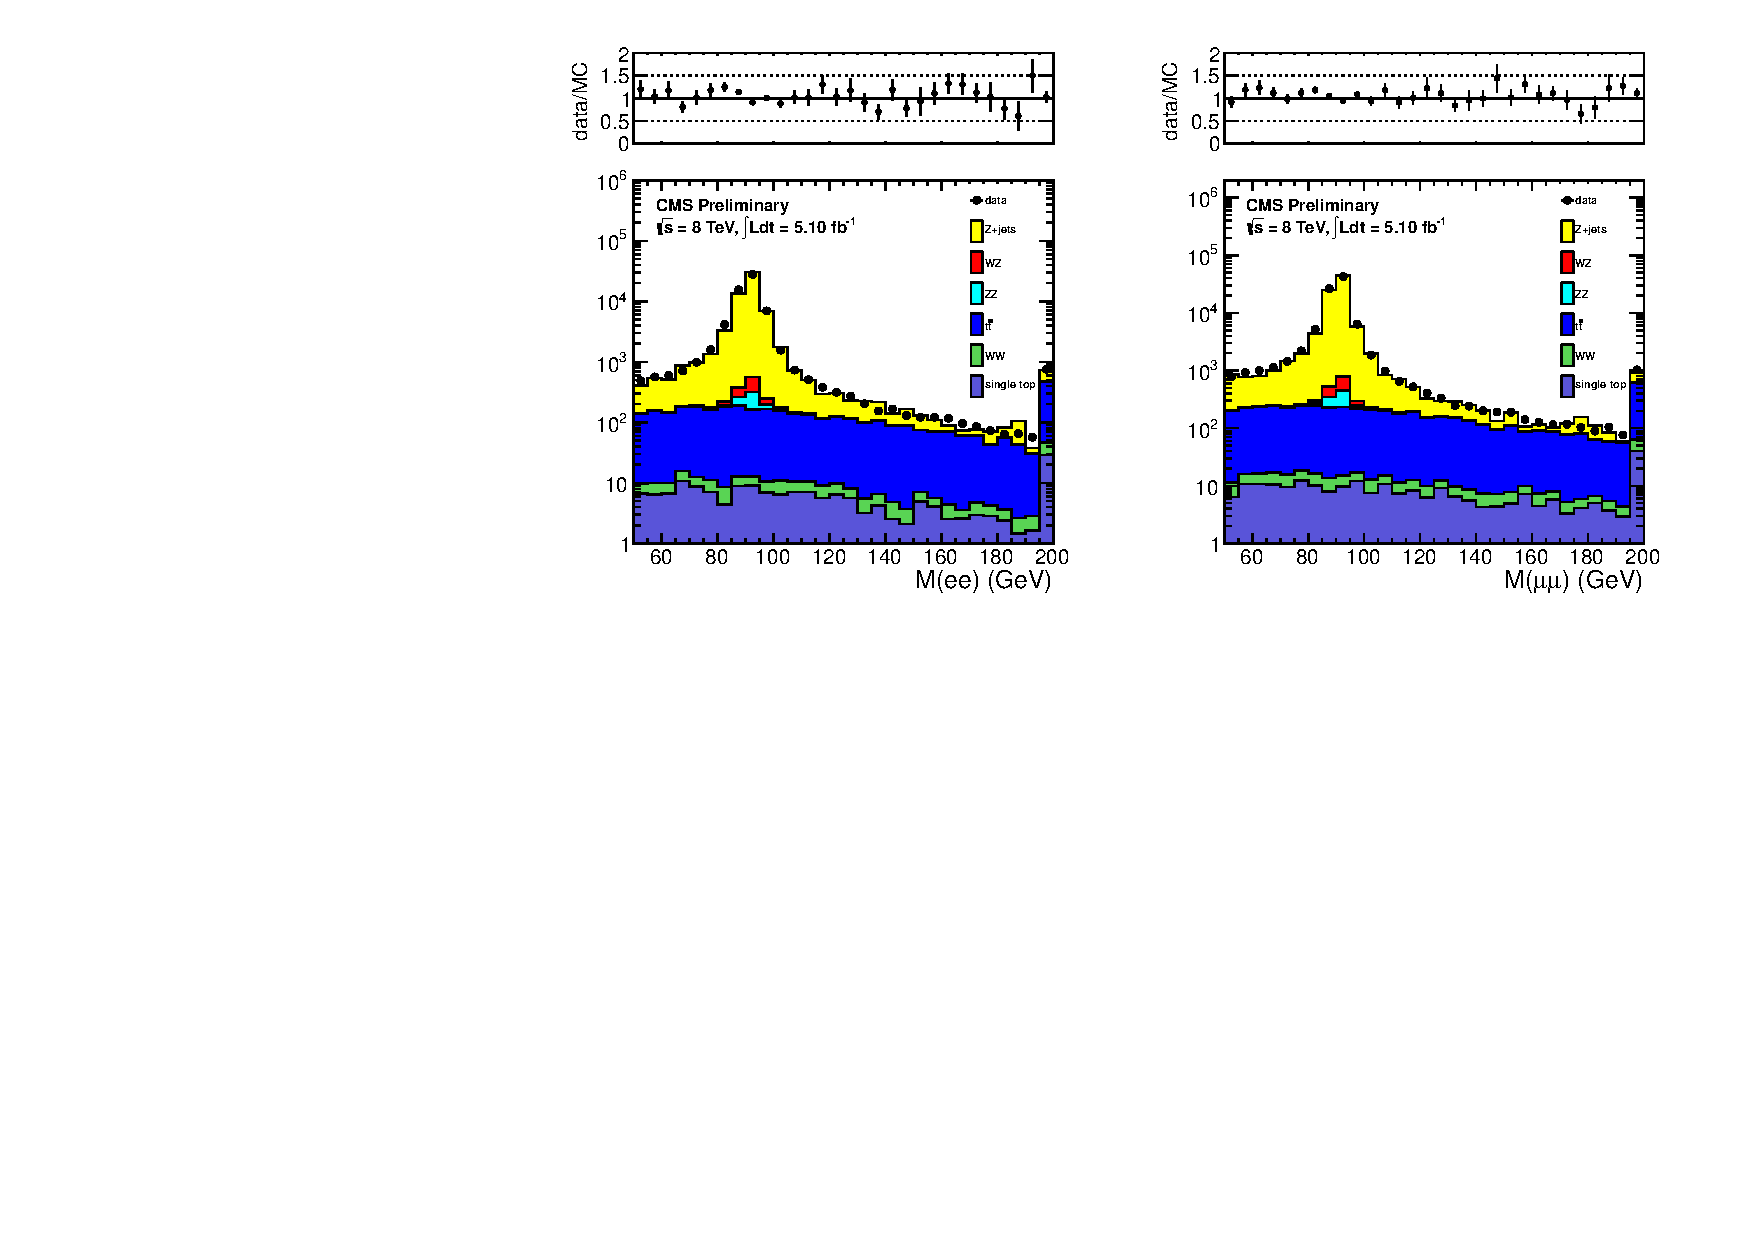
\includegraphics[width=1.0\linewidth]{plots/dilmass_ee_mm_2j.pdf}
	\caption{
	  \label{fig:dilmass_2j}\protect 
	  Dilepton mass distribution for events in the preselection region of the inclusive search
	  in the ee (left) and $\mu\mu$ (right) final states.}
  \end{center}
\end{figure}

\begin{table}[htb]
\begin{center}
\caption{\label{table:zyields_2j} Data and MC yields in the preselection region of the inclusive search.
}
\begin{tabular}{lccccc}
\hline
\hline
         Sample   &           ee   &       $\mu\mu$   &         e$\mu$   &            total  \\
\hline
          \zjets   & 53187.8 $\pm$ 988.5   &78070.5 $\pm$ 1165.7   &  5.6 $\pm$ 3.6   &131264.0 $\pm$ 1528.4  \\
          \ttbar   &   645.3 $\pm$ 17.7   &865.1 $\pm$ 19.7   &1470.4 $\pm$ 25.8   &2980.8 $\pm$ 37.0  \\
             WZ   &   431.2 $\pm$ 2.4   &594.6 $\pm$ 2.7   &  5.8 $\pm$ 0.2   &1031.6 $\pm$ 3.6  \\
             ZZ   &   269.9 $\pm$ 1.6   &377.7 $\pm$ 1.8   &  0.5 $\pm$ 0.0   &648.1 $\pm$ 2.4  \\
             WW   &    15.2 $\pm$ 0.8   & 22.2 $\pm$ 0.9   & 38.9 $\pm$ 1.3   & 76.4 $\pm$ 1.7  \\
     single top   &    28.8 $\pm$ 3.2   & 38.0 $\pm$ 3.4   & 72.0 $\pm$ 4.9   &138.8 $\pm$ 6.7  \\
\hline
    total SM MC   & 54578.1 $\pm$ 988.7   &79968.3 $\pm$ 1165.9   &1593.3 $\pm$ 26.5   &136139.7 $\pm$ 1528.9  \\
           data   &          54426   &          80367   &           1565   &         136358  \\

\hline
\hline
\end{tabular}
\end{center}
\end{table}


\clearpage

We next define the preselection region for the targeted search by adding the following requirements:
\begin{itemize}
\item Veto events containing a b-tagged jet;
\item Dijet invariant mass $70<m_{jj}<110$ GeV;
\item Veto events containing a third selected lepton (electron or muon) with \pt $>$ 20 GeV {\bf FIXME: lower third lepton \pt threshold to 10 GeV}.
\end{itemize}

The rejection of events with a b-tagged jet strongly suppresses the \ttbar\ background, which is the dominant background in the inclusive search
after requiring large \MET. The requirement that the jet pair is consistent with originating from W/Z decay is motivated by the fact that we are 
searching for signatures producing V(jj)Z($\ell\ell$)+\MET; this requirement suppresses the \zjets\ and \ttbar\ backgrounds. The veto of events
containting a third electron or muon suppresses the WZ background, and also serves to make this analyis exclusive with respect to searches in
the trilepton final state.

The dilepton mass distributions in the preselection region of the targeted search (without the dilepton mass requirement applied) 
for the ee and $\mu\mu$ final states are shown in Figure~\ref{fig:dilmass_2j_targeted}. In Table~\ref{table:zyields_2j_targeted} 
the data and MC yields in the preselection region are indicated. Good data vs. MC agreement is observed.

\begin{figure}[hbt]
  \begin{center}
	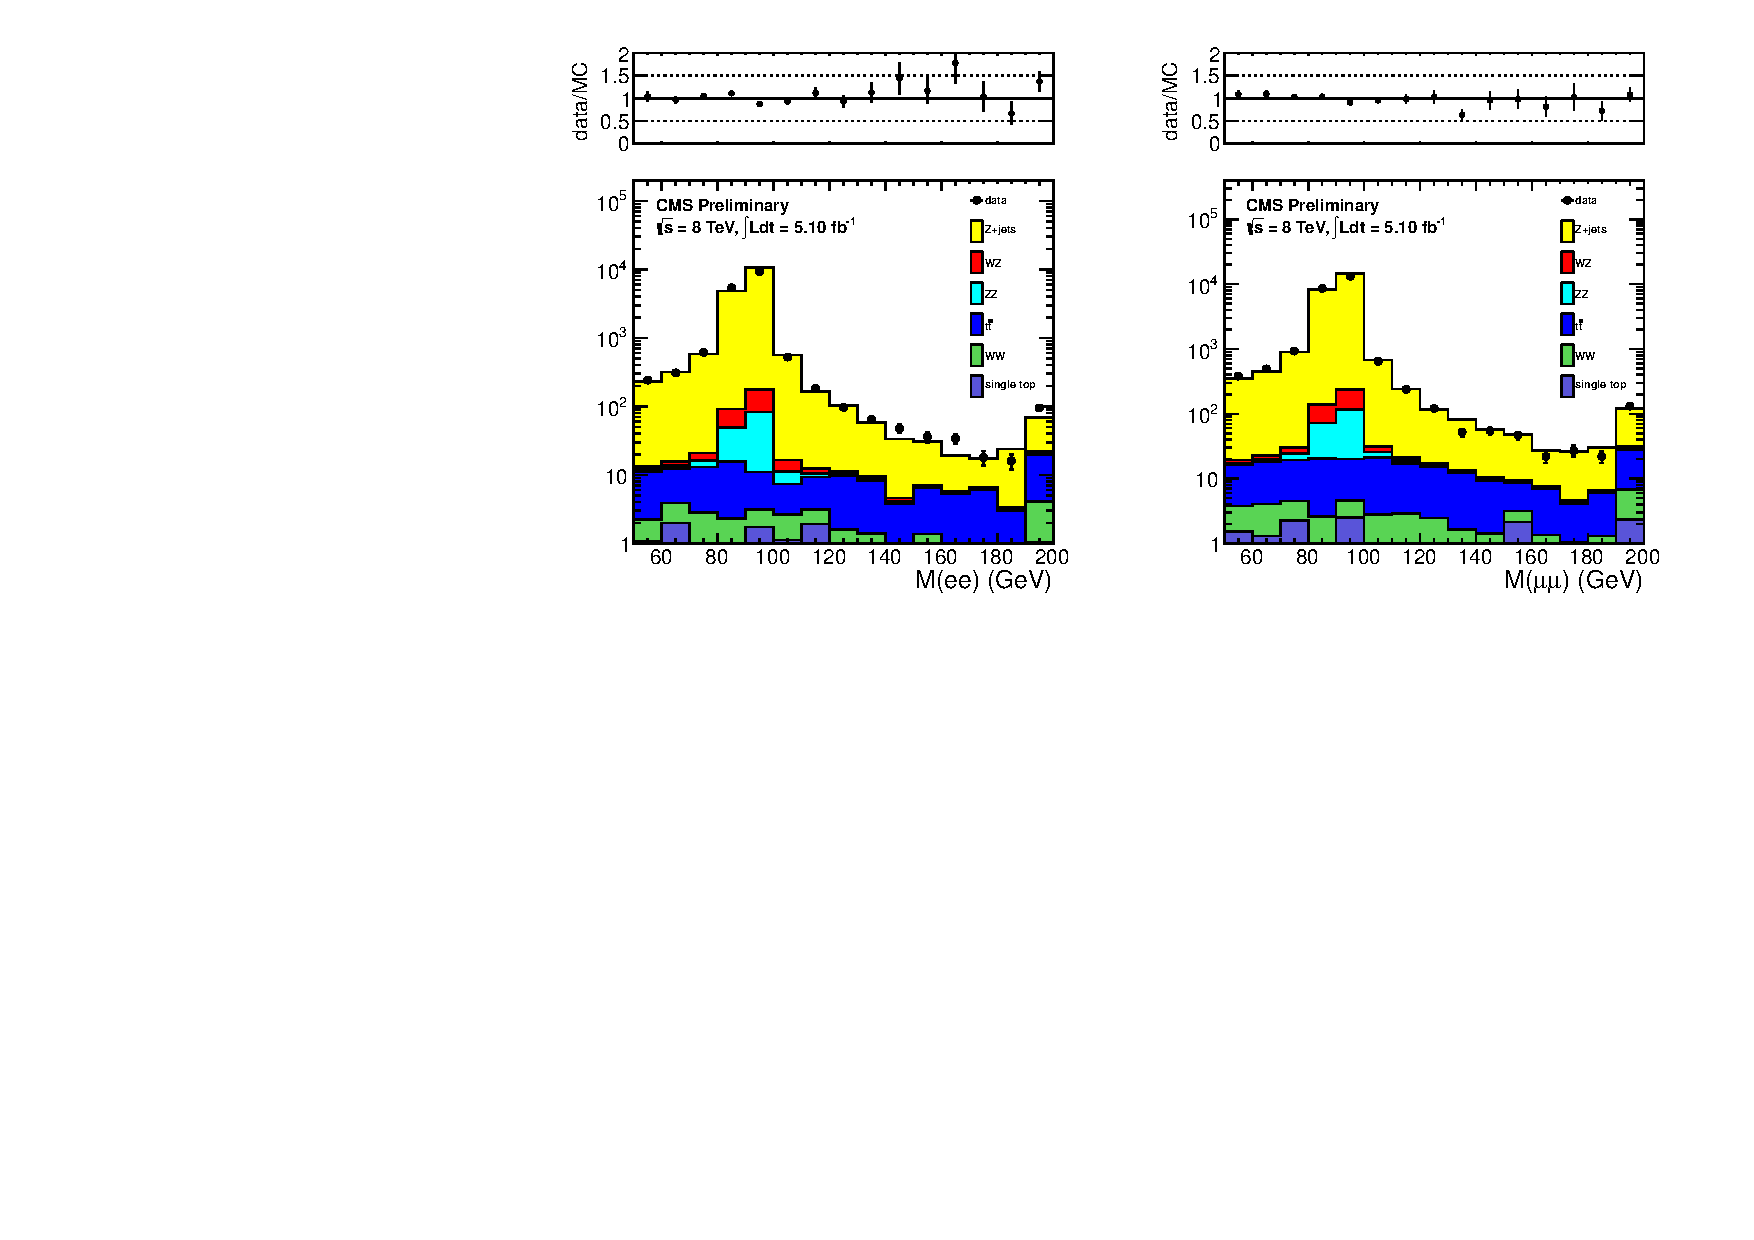
\includegraphics[width=1.0\linewidth]{plots/dilmass_ee_mm_2j_targeted.pdf}
	\caption{
	  \label{fig:dilmass_2j_targeted}\protect 
	  Dilepton mass distribution for events in the preselection region of the targeted search
	  in the ee (left) and $\mu\mu$ (right) final states.}
  \end{center}
\end{figure}

\begin{table}[htb]
\begin{center}
\caption{\label{table:zyields_2j_targeted} Data and MC yields in the preselection region of the inclusive search.
}
\begin{tabular}{lccccc}
\hline
\hline
         Sample   &           ee   &       $\mu\mu$   &         e$\mu$   &            total  \\
\hline
         \zjets   &14108.9 $\pm$ 486.3   &21927.1 $\pm$ 606.4   &  0.0 $\pm$ 0.0   &36036.0 $\pm$ 777.4  \\
         \ttbar   & 21.0 $\pm$ 2.9   & 33.4 $\pm$ 3.9   & 53.7 $\pm$ 5.0   &108.0 $\pm$ 6.9  \\
             WZ   &135.6 $\pm$ 1.4   &188.5 $\pm$ 1.6   &  1.0 $\pm$ 0.1   &325.1 $\pm$ 2.1  \\
             ZZ   &106.0 $\pm$ 1.0   &148.8 $\pm$ 1.2   &  0.1 $\pm$ 0.0   &254.9 $\pm$ 1.5  \\
             WW   &  3.4 $\pm$ 0.4   &  4.1 $\pm$ 0.4   &  7.8 $\pm$ 0.5   & 15.2 $\pm$ 0.7  \\
     single top   &  2.0 $\pm$ 0.8   &  2.8 $\pm$ 1.1   &  5.5 $\pm$ 1.4   & 10.3 $\pm$ 1.9  \\
\hline
    total SM MC   &14376.9 $\pm$ 486.3   &22304.7 $\pm$ 606.5   & 68.0 $\pm$ 5.2   &36749.6 $\pm$ 777.4  \\
           data   &          14647   &          21840   &             74   &          36561  \\
\hline
\hline
\end{tabular}
\end{center}
\end{table}


\clearpage










\begin{comment}

The data yields and the MC predictions are given in Table~\ref{preselyieldtable}.
%Dilepton mass and MET distributions for \emu ~events are shown in appendix \ref{app:emu}.

As anticipated, the MC predicts that the preselection is dominated by Z+jets in the same-flavor 
case and by \ttbar\ in the opposite-flavor case.  
%The data yield is in reasonable agreement with the predictions for the $ee$, $\mu\mu$ and $e\mu$ channels.

\begin{comment}

We also show the %LO 
next-to-leading order (NLO) 
yields for the LM4 and LM8 processes, which are benchmark
SUSY processes in which $Z$ bosons are produced via cascade decays of SUSY particles. 


\begin{table}[htb]
\begin{center}
\caption{\label{preselyieldtable} Data and Monte Carlo yields for the preselection with \njets\ $\ge$ 2 for \lumi. 
  %The NLO yields for the SUSY benchmark processes LM4 and LM8 are also shown.
}
\begin{tabular}{lccccc}
\hline
              Sample   &                $ee$   &            $\mu\mu$   &              $e\mu$   &         tot  \\
\hline

        WJets &   10.8 $\pm$    4.4  &     0.0 $\pm$    0.0  &     8.5 $\pm$    3.8  &    19.3 $\pm$    5.8 \\ 
           WW &   14.8 $\pm$    0.5  &    17.2 $\pm$    0.5  &    32.9 $\pm$    0.8  &    64.9 $\pm$    1.1 \\ 
           WZ &  405.7 $\pm$    1.8  &   411.7 $\pm$    1.7  &     5.0 $\pm$    0.1  &   822.4 $\pm$    2.5 \\ 
           ZZ &  313.3 $\pm$    1.2  &   349.1 $\pm$    1.2  &     0.8 $\pm$    0.0  &   663.2 $\pm$    1.6 \\ 
   Single Top &   29.3 $\pm$    1.2  &    26.1 $\pm$    1.0  &    50.8 $\pm$    1.5  &   106.2 $\pm$    2.1 \\ 
     \ttbar &  523.2 $\pm$    2.6  &   529.0 $\pm$    2.5  &  1056.7 $\pm$    3.6  &  2108.8 $\pm$    5.1 \\ 
       Z+Jets & 51051.4 $\pm$  147.5  &  53149.1 $\pm$  143.0  &    16.2 $\pm$    2.6  &  104216.8 $\pm$  205.4 \\ 
\hline
     Total MC & 52348.5 $\pm$  147.6  &  54482.2 $\pm$  143.0  &  1171.0 $\pm$    6.1  &  108001.6 $\pm$  205.6 \\ 
\hline
         Data &  49214  &   52757  &    1256  &  103227 \\ 
\hline


\end{tabular}
\end{center}
\end{table}

\end{comment}
